\JWlone{Methods}
\label{sec:methods}

This chapter describes how arbitrary arithmetic functions can be expressed in
terms of affine expressions. This is the most important part of this thesis
because it is the key part of evaluating arbitrary arithmetic expressions
using OAFEs \cite{davidgoliath}.


%
% ILLUSTRATION
%
\JWltwo{Illustration}
\label{sec:illustration}

This chapter informaly illustrates the key ideas and methods proposed by this
thesis. The following chapters contain a more formal bottom--up description that
is rather cumbersome to understand without grasping the overall picture.

The ultimate goal is to obliviously evaluate a polynomial by two mutual
distrusting parties. Informally, that is evaluating $f(x) = \sum a_ix^i$ where
the first party chooses $f$ and the second party chooses $x$. But neither
party should learn the choice of the other party. The naive and simple solution
is to instruct a trusted third party to evaluate the polynomial---provided by
the first party---at the grid point $x$ provided by the second party.
Of course, this solution is just as simple as insecure.

Since this thesis uses Oblivious Affine Function Evaluation (OAFE) as the main
building block, the general polynomial has to be split to affine functions
evaluating parts of the complete function. To maintain the security property,
neither party should be able to learn anything by intermediate results. The role
both parties play differs a lot: The first party---usually named \JWpOne{}---is
in possession of the function to evaluate and generates and sets up the
tamper--proof hardware token that implements the OAFE functionality. The second
party---usually named \JWpTwo{}---is less powerful: It does only evaluate
entities issued by \JWpOne{} and uses the already configured OAFEs. \JWpTwo{}
acts---if honest---completely deterministic and will receive the function's
final evaluated value.

The approach pursued here is to divide the circuit that equals the overall
function to smaller sub--circuits. Each sub--circuit can be composed of
arithmetic gates and other sub--circuts. \JWpTwo{} has to evaluate each
sub--circuit to an intermediate value. \JWpTwo{} has to store all
intermediate values since they are used to compute the following sub--circuits.
Whenever one sub--circuit $A$ contains a node that is another sub--circuit $B$,
this node gets replaced by the intermediate output value of $B$ before $A$ can
be evaluated. Obviously the intermediate values are at risk: A passively
corrupted \JWpTwo{} could try to derive information from these intermediate
results. An active \JWpTwo{} could additionally try to modify the intermediate
values and gain supplemental information out of that. To not directly reveal the
value of an evaluated sub--circuit the intermediate values have to be
\emph{encrypted}. To be able to identify an illicit modification the overall
evaluation has to fail when an attacker tries to illicitly modify an
intermediate result. In this thesis, the intermediate values are tuples of two
values. The decryption of both values represents---when well--formed---the same
value. The gain of this technique is that an attacker cannot simply change the
value and preserve the well--formedness without knowing the encryption keys. Any
chance to one (or both) tuple values causes the intermediate value to be
destroyed (formally represented as $\bot$). The value of the evaluated
polynomial is a notable exception: It's not encrypted. To derive the final
value, the output value of the last sub--circuit undergoes a special procedure.
For technical reasons both sides of the tuples are often syntactically divided
to two intermediate values that semantically still represent the same
intermediate value tuple.

\begin{figure}[htb]
  \centering
  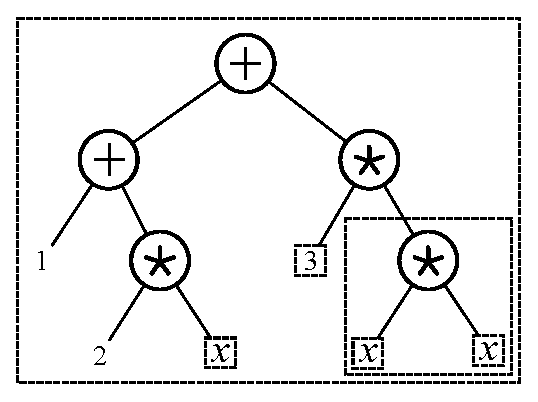
\includegraphics[width=10cm]{images/sample-polynomial.eps}
  \caption{Circuit encoding the polynomial $1 + 2x + 3x^2$ including its
    (sub--)circuits (dashed boxes)}
  \label{fig:sample-poly}
\end{figure}

The overall process is very straightforward: \JWpOne{} analyzes the polynomial
and transforms it into a circuit (the entire figure \ref{fig:sample-poly}). This
circuit is then divided to sub--circuits (every box bounded by dashes lines
except the biggest box). The evaluation order for the sample polynomial $1 + 2x
+ 3x^2$ (see figure \ref{fig:sample-poly}) is: First of all evaluate the
sub--circuit only containg $x$. This is in fact only one sub--circuit that
appears three times in the figure. The next step would be to evaluate the
sub--circuit only encoding $3$, then the sub--circuit encoding $x^2 (= x \cdot
x)$ and finally the overall circuit that encodes $1 + 2x + 3x^2$. Usually and as
in the example above, the sub--circuits are of maximal size. A sub--circuit of
maximal size is a sub--circuit into which no additional arithmetic gates can be
included. Notably, a sub--circuit can only contain multiplications that only
depend on either constants or stored intermediate values. The next step is to
set up the tamper--proof hardware token implementing the OAFE functionality.
Then, the sub--circuits along with the OAFEs are transferred to \JWpTwo{} that
evaluates the sub--circuits one after the other and uses the OAFEs in that
process. The final result will be the evaluation of the original polynomial.

To simplify the analysis of the different parts and to demonstrate the
modularity, special terms are used throughout in this thesis. A mapping from the
informal terms used above and the terms used otherwise (and defined in the
following chapters) follows:

\JWtodo{Double- und Single-Dinger besser erklären}

\begin{itemize}

  \item The overall circuit representing exactly one function is named
    \emph{Double Affine Randomized Circuit} (DRAC) and \emph{Affine Randomized
    Circuit} (RAC)---when both tuple values travel separated from each
    other---defined in chapter \ref{def:DRAC}.

  \item The sub--circuits are called \emph{Double Affine Randomized Encodings}
    (DRAE) and \emph{Randomized Affine Encodings} (RAE) defined in chapter
    \ref{def:DRAE}.

  \item The intermediate values that are encrypted twofoldly are named
    \emph{Double Randomized Affine Values} (DRAV), defined in chapter
    \ref{def:DRAV}.

\end{itemize}


%
% DEFINITIONS
%
\JWltwo{Definitions}
\label{sec:rae-definitions}

This chapter defines important entities that are used to define the more complex
entities in the following chapters.

% Field K
\JWlthree*{Field $K$}
\label{sec:field}

\label{def:field} Throughout this thesis, $K$ represents an arbitrary large
finite field, such as $\mathbb{F}_{2^{256}}$.

\JWtodo{Irreduzibled Polynom hinschreiben}


% OAFEs
\JWlthree*{OAFEs}

In this thesis the \JWdef{Oblivious Affine Function Evaluation}{OAFE}{s} are
essentially one \emph{Sequential one--time OAFE} as defined by Döttling,
Kraschewski and Müller-Quade \cite{davidgoliath}. The OAFEs can be used to
obliviously evaluate affine functions $f_i$. The collectivity of all OAFEs (as
defined in this thesis) maps to exactly one tamper--proof hardware token
realizing one \emph{Sequential one--time OAFE} \cite{davidgoliath}:

\begin{align*}
  f_i(x_i) = &
  a_ix_i + b_i \\
%
  = &
\begin{pmatrix}a_{i,1}\\a_{i,2}\\a_{i,3}\\\vdots\end{pmatrix}x_i +
\begin{pmatrix}b_{i,1}\\b_{i,2}\\b_{i,3}\\\vdots\end{pmatrix}
\end{align*}

\noindent{}Obviously, every function $f_i$ can only be evaluated only once and
the functions $f_i$ have to be evaluated in order: $f_1$ being the first, $f_2$
the second and so forth.

In this thesis usually the term OAFEs is used to denote the fact that there are
multiple affine functions ($f_i$) that can be evaluated obliviously. The term
OAFE configuration is used to denote the vectors $a_i$ and $b_i$. One OAFE
configuration is the same as the collectivity of the $(a_i, b_i, i)$ triples as
used in the original definition \cite{davidgoliath}.


%
% DUAL RANDOMIZED AFFINE VALUES
%
\JWltwo{Dual Randomized Affine Values}
\label{sec:drav}

\JWdef{Dual Randomized Affine Value}{DRAV}{s} are encrypted, signed values
representing a scalar value of the field $K$. Each DRAV is encrypted by a pair
of \emph{dual keys}. The first dual key, the \emph{static key}, remains the same
in the whole DRAC (see chapter \ref{def:DRAC}) generation procedure and is
usually denoted as $(\alpha_l, \alpha_r)$. The second dual key, the
\emph{dynamic key} is a short--lived key, usually represented as $(\beta,
\beta')$. Two DRAVs only share the same dynamic key by hazard but always share
the same static key. Encoding a regular value $v \in K$ as a DRAV
$\widetilde{v} \in \mathcal{V}_K$ is straightforward, most of the time the
universal encoding function $E(v)$ is used to describe DRAV encoding. For the
sake of simplicity $E(v)$ is already parametrized by the static dual key
$(\alpha_l, \alpha_r)$ and is able to generate a new dynamic dual key $(\beta,
\beta')$ uniformly at random. $D(\widetilde{v})$ is assumed to know the correct
decryption keys.

\begin{align*}
  \widetilde{v} = E(v) = (\widetilde{v_l}, \widetilde{v_r}) =
    (\alpha_l \cdot v + \beta, \alpha_r \cdot v + \beta')
\end{align*}

\noindent{}So, if the keys are uniformly at random, the two components of the
tuple $\widetilde{v}$ are uniformly at random, too. Decoding is (most of the
time using the universal decoding function $D(\widetilde{v})$):

\begin{align*}
  %
\begin{pmatrix}v_l\\v_r\end{pmatrix} &=
\begin{pmatrix}D_l(\widetilde{v})\\D_r(\widetilde{v})\end{pmatrix} =
  \begin{pmatrix}
    \frac{\widetilde{v_l} - \beta}{\alpha_l}\\
    \frac{\widetilde{v_r} - \beta'}{\alpha_r}
  \end{pmatrix}\\
  %
  v &= D(\widetilde{v}) =
  \left\{
    \begin{array}{l l}
      v_l & \quad \text{if}~v_l = v_r\\
      \bot & \quad \text{otherwise ($\widetilde{v}$ is non--well--formed)}\\
    \end{array}\right.
\end{align*}

\begin{lem}
  \label{lem:DRAV-random}

  A party that is not in posession of the encrytion (dual) keys will not learn
  anything from a DRAV. A DRAV is a tuple consisting of two values uniformly at
  random that is uncorrelated to any other DRAV.

\end{lem}
\begin{proof}

  In a finite field, the addition of some value $r$ uniformly at random to
  another value $x \in K$ is uniformly at random. Therefore $\alpha_l \cdot v +
  \beta$ and $\alpha_r \cdot v + \beta'$ are two values uniform at random if and
  only if $\beta$ and $\beta'$ are uniformly at random. Per definition of a
  DRAV, everytime a DRAV gets encoded, $\beta$ and $\beta'$ are fresh uniformly
  distributed random values. Trivially, a DRAV is uncorrelated to any other
  DRAV.

\end{proof}


% WELL-FORMED DRAVs
\JWlthree{Well--Formed DRAVs}

A DRAV $\widetilde{v}$ is well--formed iff $D(\widetilde{v}) \neq \bot$.
Therefore, if $D(\widetilde{\chi}) = \bot$, $\chi$ is non--well-formed.
Obviously the well--formedness of a DRAV depends on the encryption keys using
which it gets decrypted. Decoding a well--formed DRAVs using any other decoding
function will lead to $\bot$ because the well--formed DRAV looks
non--well--formed to the other decoding function.

\begin{lem}
  \label{lem:well-formed-fun-of-dec-fun}

  DRAV well--formedness is a function of the decryption function used to decrypt
  it.

\end{lem}
\begin{proof}

  Assuming two well--formed DRAVs $\widetilde{a}$ and $\widetilde{b}$. Both
  DRAVs have their respective decoding function $D^a$ and $D^b$ and their
  dynamic dual key (say $\beta_1$ and $\beta_2$ for $\widetilde{a}$ and
  $\beta_3$ and $\beta_4$ for $\widetilde{b}$).

  \begin{align*}
    %
    D^a(\widetilde{a}) &= D(\widetilde{a}) \qquad\text{(using $\widetilde{a}$'s
    keys)}\\
    %
    D^b(\widetilde{b}) &= D(\widetilde{b}) \qquad\text{(using $\widetilde{b}$'s
    keys)}\\
    %
    a &= D^a(\widetilde{a}) \hat{=}
    \begin{pmatrix}
      \frac{(\alpha_l \cdot a + \beta_1) - \beta_1}{\alpha_l}\\
      \frac{(\alpha_r \cdot a + \beta_2) - \beta_2}{\alpha_r}\\
    \end{pmatrix}
    = a\\
    %
    a' &= D^a(\widetilde{b}')
    \hat{=}
    \begin{pmatrix}
      \frac{(\alpha_l \cdot b + \beta_3) - \beta_1}{\alpha_l}\\
      \frac{(\alpha_r \cdot b + \beta_4) - \beta_2}{\alpha_r}\\
    \end{pmatrix}
    \hat{=}
    \begin{pmatrix}
      b +
      \frac{\beta_3 - \beta_1}{\alpha_l}\\
      b +
      \frac{\beta_4 - \beta_2}{\alpha_r}\\
    \end{pmatrix}
    = \bot\\
    %
    b &= D^b(\widetilde{b}) \hat{=}
    \begin{pmatrix}
      \frac{(\alpha_l \cdot b + \beta_3) - \beta_3}{\alpha_l}\\
      \frac{(\alpha_r \cdot b + \beta_4) - \beta_4}{\alpha_r}\\
    \end{pmatrix}
    = b\\
    %
    b' &= D^b(\widetilde{a}')
    \hat{=}
    \begin{pmatrix}
      \frac{(\alpha_l \cdot a + \beta_1) - \beta_3}{\alpha_l}\\
      \frac{(\alpha_r \cdot a + \beta_2) - \beta_4}{\alpha_r}\\
    \end{pmatrix}
    \hat{=}
    \begin{pmatrix}
      a +
      \frac{\beta_1 - \beta_3}{\alpha_l}\\
      a +
      \frac{\beta_2 - \beta_4}{\alpha_r}\\
    \end{pmatrix}
    = \bot\\
    %
  \end{align*}

  As one can see decoding a well--formed DRAV using the wrong decoding function
  leads to $\bot$.
\end{proof}


\begin{lem}
  \label{lem:DRAV-indistinguishable}

  Without knowing the encryption keys, a non--well--formed DRAV is
  indistinguishable from a well--formed DRAV.

\end{lem}
\begin{proof}

  From Lemma \ref{lem:DRAV-random} we learn, that a well--formed DRAV only
  consists of two values uniformly at random. From Lemma
  \ref{lem:well-formed-fun-of-dec-fun} we learn, that well--formedness is a
  function of the encryption keys used to eventually decrypt the DRAV. Since a
  party that is not in posession of the encryption keys cannot know the
  decryption function, well--formed and non--well--formed DRAVs are
  indistinguishable for a party not in posession of the keys.
\end{proof}


% DIRECT DRAV ARITHMETIC
\JWlthree{Direct DRAV Arithmetic}
\label{sec:direct-DRAV-arithmetic}

Direct DRAV arithmetic only supports addition ($+$) of two DRAVs. Indirect DRAV
arithmetic has to be used for other operations. The advantage of direct DRAV
arithmetic is that it can be performed without the knowledge of a DRAV's
encryption keys. But (see Lemma \ref{lem:wrong-add}) the addition of DRAVs does
not lead to additional information except when intented by a party in possession
of the encryption keys.

\begin{lem}
  \label{lem:DRAV-add}

Additions commissioned by a party in possession of the encryption keys of
well--formed DRAVs lead to well--formed DRAV: $\widetilde{x} =
(\widetilde{x_l}, \widetilde{x_r})$ and $\widetilde{y} = (\widetilde{y_l},
\widetilde{y_r})$ can be added componentwise to $\widetilde{z} =
\left(\widetilde{x_1} + \widetilde{y_1}, \widetilde{x_2} +
\widetilde{y_2}\right)$. The encryption keys for $\widetilde{z}$ will be
$(\alpha_l, \alpha_r)$ and $(\beta_1 + \beta_3, \beta_2 + \beta_4)$ assuming
$\widetilde{x}$ was encrypted with $(\alpha_l, \alpha_r)$ and $(\beta_1,
\beta_2)$ and $y$ was encrypted with $(\alpha_l, \alpha_r)$ and $(\beta_3,
\beta_4)$.

\end{lem}
\begin{proof}

From ($\widetilde{x} = \left(\alpha_l \cdot x + \beta_1,
\alpha_r \cdot x + \beta_2\right)$, $\widetilde{y} = \left(\alpha_l \cdot x +
\beta_3, \alpha_r \cdot x + \beta_4\right)$) it's obvious that: $\widetilde{z} =
\left(\alpha_l \cdot (x+y) + (\beta_1 + \beta_3), \alpha_r \cdot (x+y) +
(\beta_2 + \beta_4)\right)$ and $\widetilde{z}$ is well--formed.

\end{proof}

\begin{lem}
  \label{lem:DRAV-add-bad}

The addition to a non--well--formed DRAV leads to a non--well--formed DRAV. It's
of particular interest the following property holds: $\forall \widetilde{x}:
\widetilde{x} + \bot = \bot + \widetilde{x} = \bot$.

\end{lem}
\begin{proof}

Let $\widetilde{\chi}$ be a
non--well--formed DRAV, so: $\widetilde{\chi} = (\alpha_l \cdot \chi + \beta_3 +
\Delta_l, \alpha_r \cdot \chi + \beta_4 + \Delta_r)$. The component--wise
addition $\widetilde{\nu}$ of $\widetilde{\chi}$ to any well--formed
$\widetilde{x} = (\alpha_l \cdot x + \beta_1, \alpha_r \cdot x + \beta_2)$ is
$\widetilde{\nu} = (\alpha_l \cdot (x+\chi) + (\beta_1+\beta_3) + \Delta_l,
\alpha_r \cdot (x+\chi) + (\beta_2+\beta_4) + \Delta_r)$. Using the universal
decoding function $D$, the value of $\chi$ is $\chi = D(\widetilde{\chi}) = (x +
\chi + \frac{\Delta_l}{\alpha_l}, x + \chi + \frac{\Delta_r}{\alpha_r})$. So:
$\forall (\Delta_r, \Delta_l) \in K \setminus \{(0, 0)\} \wedge
\frac{\Delta_l}{\alpha_l} \neq \frac{\Delta_r}{\alpha_r}: D(\widetilde{\chi}) =
\bot$. Since the encryption keys are not known to an attacker,
$\frac{\Delta_l}{\alpha_l} \neq 0 \wedge \frac{\Delta_r}{\alpha_r}$ hold except
for a negligible probability if $\Delta_r \neq 0 \vee \Delta_r \neq 0$ and
that's the property for being forged (non--well--formed) which was the
assumption. Trivially $\bot + \bot = \bot$ by a similar argument.

\end{proof}


\begin{lem}
  \label{lem:wrong-add}

  The addition that was unintended by a party in possession of the encryption
  keys will not reveal additional informaion. A party that is not in possession
  of the keys but knows three well--formed DRAVs $\widetilde{a}$,
  $\widetilde{b}$ and $\widetilde{c}$ that is commissioned to execute the
  addition $\widetilde{y} = \widetilde{a} + \widetilde{b}$ cannot generate a
  well--formed DRAV $\widetilde{y}' = \widetilde{a} + \widetilde{c}$.

\end{lem}

\begin{proof}

  Since every DRAV has per definition different dynamic keys the
  component--wise addition of two DRAVs leads to a new dynamic key that is
  characteristic for the addition intended by a party in possession of the
  encruption keys.

  Assuming there are three well--formed DRAVs $\widetilde{a}$, $\widetilde{b}$
  and $\widetilde{c}$ and the party in possession of the keys commissiones any
  other party to execute $\widetilde{y} = \widetilde{a} + \widetilde{b}$ but the
  other party tries to illicitly execute $\widetilde{y}' = \widetilde{a} +
  \widetilde{c}$:

  \begin{align*}
    %
    \widetilde{a} &=
    \begin{pmatrix}
      \alpha_l \cdot a + \beta_1\\
      \alpha_r \cdot a + \beta_2
    \end{pmatrix}\\
    %
    \widetilde{b} &=
    \begin{pmatrix}
      \alpha_l \cdot b + \beta_3\\
      \alpha_r \cdot b + \beta_4
    \end{pmatrix}\\
    %
    \widetilde{c} &=
    \begin{pmatrix}
      \alpha_l \cdot c + \beta_5\\
      \alpha_r \cdot c + \beta_6
    \end{pmatrix}\\
    %
    \widetilde{y} &=
    \begin{pmatrix}
      \alpha_l \cdot a + \beta_1 + \alpha_l \cdot b + \beta_3\\
      \alpha_r \cdot a + \beta_2 + \alpha_r \cdot b + \beta_4\\
    \end{pmatrix} =
    \begin{pmatrix}
      \alpha_l \cdot (a+b) + (\beta_1 + \beta_3)\\
      \alpha_r \cdot (a+b) + (\beta_2 + \beta_4)\\
    \end{pmatrix}\\
    %
    \widetilde{y}' &=
    \begin{pmatrix}
      \alpha_l \cdot a + \beta_1 + \alpha_l \cdot c + \beta_5\\
      \alpha_r \cdot a + \beta_2 + \alpha_r \cdot c + \beta_6\\
    \end{pmatrix} =
    \begin{pmatrix}
      \alpha_l \cdot (a+c) + (\beta_1 + \beta_5)\\
      \alpha_r \cdot (a+c) + (\beta_2 + \beta_6)\\
    \end{pmatrix}\\
    %
  \end{align*}

  As soon as the party in possession of the keys tries to decode using the
  encryption keys for $\widetilde{y}$ the result (either $\widetilde{y}$ or
  $\widetilde{y}'$) the other party will get caught if it tried to cheat:

  \begin{align*}
    %
    D^y(\widetilde{y}) &= D(y) \qquad\text{(using $y$'s encryption keys)}\\
    %
    y &= D^y(\widetilde{y}) \hat{=}
    \begin{pmatrix}
      \frac{(\alpha_l \cdot (a+b) + (\beta_1 + \beta_3)) - (\beta_1+\beta_3)}
           {\alpha_l}\\
      \frac{(\alpha_r \cdot (a+b) + (\beta_2 + \beta_4)) - (\beta_2+\beta_4)}
           {\alpha_r}\\
    \end{pmatrix}
    = a+b\\
    %
    y' &= D^y(\widetilde{y}')
    \hat{=}
    \begin{pmatrix}
      \frac{(\alpha_l \cdot (a+b) + (\beta_1 + \beta_5)) - (\beta_1+\beta_3)}
           {\alpha_l}\\
      \frac{(\alpha_r \cdot (a+b) + (\beta_2 + \beta_6)) - (\beta_2+\beta_4)}
           {\alpha_r}\\
    \end{pmatrix}
    \hat{=}
    \begin{pmatrix}
      (a+b) +
      \frac{\beta_5 - \beta_3}{\alpha_l}\\
      (a+b) +
      \frac{\beta_6 - \beta_4}{\alpha_r}\\
    \end{pmatrix}
    = \bot\\
  \end{align*}
\end{proof}


% INDIRECT DRAV ARITHMETIC
\JWlthree{Indirect DRAV Arithmetic}
\label{sec:indirect-DRAV-arithmetic}

Indirect DRAV arithmetic assumes the universal encoding and decoding functions
$E(v)$ and $D(\widetilde{v})$ and therefore the knowledge of the encryption
keys. Another possibility is to map indirect DRAV arithmetic to OAFE calls that
are set up by a party that knows the encryption keys.

Indirect DRAV arithmetic is straightforward but can only be performed by a party
in possession of the encryption keys. For any operator $\odot$, $\widetilde{a}
\odot \widetilde{b} = E(D(\widetilde{a}) \odot D(\widetilde{b}))$. Obviously
it's important that $\forall x: \bot \odot x = x \odot \bot = \bot$. $\bot$ can
be represented as a DRAV as a tuple that is made up of two values uniform at
random.


% FINAL DRAV DECODING
\JWlthree{Final DRAV Decoding}
\label{sec:drav-final-decoding}

Finally decoding a DRAV can be trivially done using the universal decoding
function $D(\widetilde{v})$. But $D$ is only available to a party that is in
possession of the encryption keys.

Additionally a DRAV can also be finally decoded only one additional OAFE call.
The following procedure will decode a DRAV to a final scalar value although
$D$ is a partial function. To enable a second party---that is not in possession
of the encryption keys---to decode a DRAV $\widetilde{v} = (\widetilde{v_1},
\widetilde{v_2})$, the first party---in possession of the keys---needs to set up
a special OAFE, called the \emph{final OAFE} below.

The second party's input to the final OAFE is $\widehat{v} = \widetilde{v_1} +
\widetilde{v_2}$, the addition of both components of the DRAV to decode.  The
final OAFE was set up by the first party as follows: Assuming $\widetilde{v}$ is
encrypted by $(\alpha_l, \alpha_r)$ and $(\beta_1, \beta_2)$ the first party
knows $\widehat{v}$ has to be encrypted using $(\alpha_l + \alpha_r)$ and
$(\beta_1 + \beta_2)$.  Given this knowledge the final OAFE setup is
$\frac{1}{\alpha_l + \alpha_r} \cdot \widehat{v} - \frac{\beta_1 +
\beta_2}{\alpha_l + \alpha_r}$.

Again, it's important that an attacker is getting caught when trying to forge a
DRAV ($D(\widetilde{v}) = \bot$ if $\widetilde{v}$ has been forged, $\bot$ is
mapped to uniform randomness in this process since an OAFE has no
$\bot$--value). If the attacker cheated somewhere in the process and forged one
of the DRAV tuples $\widetilde{x} = (\widetilde{x_1}, \widetilde{x_2})$ to
$\widetilde{x'} = (\widetilde{x_1} + \Delta_1, \widetilde{x_2} + \Delta_2)$, the
DRAV $\widetilde{x'}$ becomes---except for a negligible
probability---non--well--formed (see section \ref{sec:drav}). The result is that
the decoded result will become uniform randomness (assuming $\widetilde{x}$ is
forged to $\widetilde{x'_1} = \widetilde{x_1} + \Delta_1$ and $\widetilde{x'_2}
= \widetilde{x_2} + \Delta_2$):

\begin{align*}
  \widehat{x'} = & \widetilde{x'_1} + \widetilde{x'_2} = \widetilde{x_1} +
  \Delta_1 + \widetilde{x_2} + \Delta_2 \\
  %
  \Rightarrow x' = & \frac{1}{\alpha_l + \alpha_v} \cdot \widehat{x'} -
  \frac{\beta_{x_1} +
  \beta_{x_2}}{\alpha_l + \alpha_v} \\
  %
  \Leftrightarrow x' = & \frac{\widetilde{x_1} + \Delta_1 +
  \widetilde{x_2} + \Delta_2}{\alpha_l + \alpha_v} -
  \frac{\beta_{x_1} +\beta_{x_2}}{\alpha_l + \alpha_v}\\
  %
  \Leftrightarrow x' = & \frac{(\alpha_l x + \beta_{x_1}) + \Delta_1 +
  (\alpha_v x + \beta_{x_2}) + \Delta_2}{\alpha_v + \alpha_l} -
  \frac{\beta_{x_1} +\beta_{x_2}}{\alpha_l + \alpha_v} \\
  %
  \Leftrightarrow x' = & \frac{(\alpha_l+\alpha_v)x + (\beta_{x_1}+\beta_{x_2} +
  \Delta_1+\Delta_2)}{\alpha_l+\alpha_v} -
  \frac{\beta_{x_1} +\beta_{x_2}}{\alpha_l + \alpha_v} \\
  %
  \Leftrightarrow x' = & x + \frac{\beta_{x_1}+\beta_{x_2}}{\alpha_l+\alpha_v}
  + \frac{\Delta_1 + \Delta_2}{\alpha_l + \alpha_v} -
  \frac{\beta_{x_1}+\beta_{x_2}}{\alpha_l + \alpha_v} \\
  %
  \Leftrightarrow x' = & x + \frac{\Delta_1 + \Delta_2}{\alpha_l + \alpha_v}\\
\end{align*}

Because an attacker is not in possession of the static encryption keys
$\alpha_l$ and $\alpha_r$, it cannot control the value of $\frac{\Delta_1 +
\Delta_2}{\alpha_l + \alpha_r}$. Since $\alpha_l$ and $\alpha_r$ are chosen
uniform at random, the result $x'$ becomes uniform at random, too. An attacker
could choose $\Delta_l + \Delta_r = 0$ but that would not change the result at
all.


%
% DUAL RANDOMIZED AFFINE ENCODING
%
\JWltwo{Dual Randomized Affine Encoding}
\label{sec:drae}

\JWdef{Dual Randomized Affine Encoding}{DRAE}{s} are affine representations of
parts of arithmetic circuits that fulfill several properties:

\begin{enumerate}

  \item \label{prop:drae-encrypted} DRAEs are encrypted: Without the encryption
    keys, they don't reveal any information.

  \item \label{prop:drae-signed} DRAEs are signed: If someone tries to forge a
    DRAE, it will become non--well--formed and operations with that DRAE result
    in non--well--formed DRAEs.

  \item \label{prop:drae-oafe} DRAEs can be securely evaluated using OAFEs.

  \item \label{prop:drae-not-enough} DRAEs can not express arbitrary arithmetic
    circuits alone.

\end{enumerate}

\noindent{}A DRAE can be eventually evaluated to a final value, that is a DRAV
(see chapter \ref{def:DRAV}). Informally, a DRAE is composed of two finite
multi--sets. The first multi--set, called the \emph{multiplicative terms}
contains tuples of computations. The second multi--set, called the
\emph{additive terms} contains computations that can be evaluated to DRAVs. The
component--wise multiplication of each of the computation tuples (from the
multiplicative terms) yields DRAVs, too. The addition of all the DRAVs obtained
from the additive terms and all the DRAVs obtained from the multiplicative terms
leads to a DRAV that is the evaluation of this DRAE.

More formally, a DRAE can be described as follows where $\mathcal{E}$ represents
the DRAEs, $\mathcal{C}$ the computations and $\mathcal{V}_\mathcal{C}$ the
computations that lead to DRAVs.

\begin{align}
%
  &\text{The static keys } \alpha_l, \alpha_r \in K \setminus \{0\} \nonumber\\
%
  &\text{The dynamic keys } \beta, \beta' \in K \nonumber\\
%
  &s, x, x', i \in K \nonumber\\
%
  \mathcal{C} = & \{ c(x) = s \cdot x + i \} \nonumber\\
%
  \mathcal{V}_\mathcal{C} = & \{ (\alpha_l \cdot f(x) + \beta,
                      \alpha_r \cdot f'(x') + \beta' )
                    \mid f, f' \in \mathcal{C} \} \nonumber\\
%
  \label{rel:DRAE}
  \mathcal{E}_\mathcal{C} = & \{ (M, A) \mid
      M \subseteq \mathcal{V}_\mathcal{C} \times
      \mathcal{V}_\mathcal{C}, A \subseteq, \mathcal{V}_\mathcal{C};
  A, M~\text{finite multi--sets} \}
%
\end{align}

Pre--evaluating a DRAE to DRAVs can be done by evaluating the OAFEs set up by
the party in possession of the encryption keys. Obviously none of the
computations $c \in \mathcal{C}$ becomes visible by the party not in possession
of the keys. The latter party will only learn exactly one evaluation $c(x)$ for
each variable $x$. This leads to pre--evaluated DRAEs of the form

\begin{align}
  \mathcal{V} = & \{ (v_l, v_r) \mid v_l, v_r \in K \}
  \text{, the DRAVs (chapter \ref{def:DRAV})} \nonumber\\
%
  \label{rel:pre-eval-DRAE}
  \mathcal{E} = & \{ (M, A) \mid
      M \subseteq \mathcal{V} \times \mathcal{V}, A \subseteq, \mathcal{V} \}
      \text{, the pre--evaluated DRAEs}
\end{align}

Evaluating a pre--evaluated DRAE is straightforward: A DRAE $e \in \mathcal{E} =
(M,A)$ can be evaluated to its single resulting DRAV $r \in \mathcal{V}$ as
follows (all additions performed component--wise):

\begin{align*}
M' &= \Bigg\{ m_1 \cdot m_2\ \Bigg|\ \begin{pmatrix}m_1\\m_2\end{pmatrix}
\in M \Bigg\} \\
r & = \sum_{a \in A}a + \sum_{m \in M'}m
\end{align*}


% DRAE ARITHMETIC
\JWlthree{DRAE Arithmetic}

%Direct Addition
\JWlfour{Addition}

Since two DRAVs can directly be added as explained in chapter
\ref{sec:direct-DRAV-arithmetic}, two DRAEs can be added by concatenating the
multiplicative ($M$ in relations \ref{rel:DRAE} and \ref{rel:pre-eval-DRAE}) and
additive ($A$) terms. Notably, although the encryption keys change, this
operation can be performed by any party, in possession of the encryption keys or
not. Obviously, the same argument holds for pre--evaluated DRAEs.


%Indirect Addition
\JWlfour{Indirect Addition via OAFEs}

The indirect addition of $\widetilde{z} = \widetilde{x_1} + \widetilde{x_2}$ is
$\widetilde{z} =
\left( E\left(D_l(\widetilde{x}) + D_l(\widetilde{y})\right),
       E\left(D_r(\widetilde{x}) + D_r(\widetilde{y})\right)
\right)$
(see chapter \ref{sec:indirect-DRAV-arithmetic}).
Since $E(x)$ and $D(x)$ are both linear functions, $E\left(D(\ldots)
+D(\ldots)\right)$ are linear functions, too that can be evaluated using two
OAFE calls.  Obviously the OAFEs have to be configured appropriately by the
party in possession of the encryption keys.


%Multiplication
\JWlfour{Multiplication}
\label{sec:DRAE-multiplication}

As described in chapter \ref{def:DRAV}, DRAV cannot be multiplied directly.
Therefore DRAVs have to be multiplied indirectly requiring additional OAFE
calls. To maintain the important DRAV and DRAE property that any operation on
bottom ($\bot$) results in bottom, the two components of each DRAV get mixed for
multiplication.

\JWtodo{Warum müssen sie gemixt werden: Das Argument mit gegen
Null prüfen}

\JWtodo{Das Mixen genauer erklären}


\begin{align*}
  E & \in \mathcal{E}; \widetilde{x}, \widetilde{y} \in \mathcal{V};
  r_1, r_2, r_3, r_4, r_5, r_6, r_7, r_8 \in K;
  \alpha_l, \alpha_r \in K \setminus \{0\} \\
  %
  E & = \widetilde{x} \cdot \widetilde{y} \\
  %
  E & = \Bigg(\left\{\left(
            \begin{pmatrix}
              \alpha_l \cdot D_l(\widetilde{x}) - r_1 \\
              \alpha_r \cdot D_r(\widetilde{x}) - r_5
            \end{pmatrix},
            \begin{pmatrix}
              1        \cdot D_l(\widetilde{y}) - r_2 \\
              1        \cdot D_r(\widetilde{y}) - r_6
            \end{pmatrix}
        \right)\right\}, \\
    &   \qquad\bigg\{
        \begin{pmatrix}
            \alpha_lr_2 \cdot D_r(\widetilde{x}) + r_3 \\
            \alpha_rr_6 \cdot D_l(\widetilde{x}) + r_7
          \end{pmatrix} \\
    &  \qquad,
        \ \begin{pmatrix}
            r_1        \cdot D_r(\widetilde{y}) + r_4 \\
            r_5        \cdot D_l(\widetilde{y}) + r_8
          \end{pmatrix}
        \bigg\}\Bigg) \\
\end{align*}

Decoding (see chapter \ref{def:DRAE}) a possibly non--well--formed $E$ to
$\widetilde{e} \in \mathcal{V}$ leads to:

\begin{align*}
  \widetilde{e} & =
  \begin{pmatrix}
    (\alpha_l D_l(\widetilde{x})-r_1)
    (         D_l(\widetilde{y})-r_2) \\
    (\alpha_r D_r(\widetilde{x})-r_5)
    (         D_r(\widetilde{y})-r_6)
  \end{pmatrix}
  +
  \begin{pmatrix}
    \alpha_lr_2 D_r(\widetilde{x}) + r_3 +
    r_1         D_r(\widetilde{y}) + r_4 \\
    \alpha_rr_6 D_l(\widetilde{x}) + r_7 +
    r_5         D_l(\widetilde{y}) + r_8
  \end{pmatrix} \\
%
  & =
  \begin{pmatrix}
    \alpha_l     D_l(\widetilde{x}) D_l(\widetilde{y})
    -\alpha_lr_2 D_l(\widetilde{x})
    -r_1         D_l(\widetilde{y})
    +r_1r_2 \\
    \alpha_r     D_r(\widetilde{x}) D_r(\widetilde{y})
    -\alpha_rr_6 D_r(\widetilde{x})
    -r_5         D_r(\widetilde{y})
    +r_5r_6
  \end{pmatrix} \\
  &\ \ \ +
  \begin{pmatrix}
    \alpha_lr_2 D_r(\widetilde{x}) + r_3 +
    r_1         D_r(\widetilde{y}) + r_4 \\
    \alpha_rr_6 D_l(\widetilde{x}) + r_7 +
    r_5         D_l(\widetilde{y}) + r_8
  \end{pmatrix} \\
%
  & =
  \begin{pmatrix}
    \alpha_l     \left(x + \frac{\Delta_1}{\alpha_l}\right)
                 \left(y + \frac{\Delta_3}{\alpha_l}\right)
    -\alpha_lr_2 \left(x + \frac{\Delta_1}{\alpha_l}\right)
    -r_1         \left(y + \frac{\Delta_3}{\alpha_l}\right)
    +r_1r_2 \\
    \alpha_r     \left(x + \frac{\Delta_2}{\alpha_r}\right)
                 \left(y + \frac{\Delta_4}{\alpha_r}\right)
    -\alpha_rr_6 \left(x + \frac{\Delta_2}{\alpha_r}\right)
    -r_5         \left(y + \frac{\Delta_4}{\alpha_r}\right)
    + r_5r_6
  \end{pmatrix} \\
  &\ \ \ +
  \begin{pmatrix}
    \alpha_lr_2  \left(x + \frac{\Delta_2}{\alpha_r}\right) + r_3 +
    r_1          \left(y + \frac{\Delta_4}{\alpha_r}\right) + r_4 \\
    \alpha_rr_6  \left(x + \frac{\Delta_1}{\alpha_l}\right) + r_7 +
    r_5          \left(y + \frac{\Delta_3}{\alpha_l}\right) + r_8
  \end{pmatrix} \\
%
  & =
  \begin{pmatrix}
    \alpha_l(xy) + (r_1r_2 + r_3 + r_4)
    + \Delta_3x + \Delta_1y
    + \frac{\Delta_1\Delta_3}{\alpha_l}
    - \Delta_1r_2
    + \frac{\Delta_2\alpha_lr_2}{\alpha_r}
    - \frac{\Delta_3r_1}{\alpha_l}
    + \frac{\Delta_4r_1}{\alpha_r}
    \\
    \alpha_r(xy) + (r_5r_6 + r_7 + r_8)
    + \Delta_4x + \Delta_2y
    + \frac{\Delta_2\Delta_4}{\alpha_l}
    + \frac{\Delta_1\alpha_lr_6}{\alpha_r}
    - \Delta_2r_6
    + \frac{\Delta_3r_5}{\alpha_r}
    - \frac{\Delta_4r_5}{\alpha_l}
  \end{pmatrix} \\
%
\end{align*}

\noindent{}That leads to two possibilities: Either $E$ is well--formed or not.

\paragraph{The DRAVs $\widetilde{x}$ and $\widetilde{y}$ are well--formed}

This leads to a DRAV encoding the desired result $E(x \cdot y)$. The resulting
encryption keys for $\widetilde{e}$ are $\alpha_l$, $\alpha_r$ (static keys) and
$\beta = r_1r_2 + r_3 + r_4$, $\beta' = r_5r_6 + r_7 + r_8$ (dynamic keys).

\begin{align*}
  %
  \Delta_1=\Delta_2=\Delta_3=\Delta_4=0 \Rightarrow
  \widetilde{e} =
  \begin{pmatrix}
    \alpha_l(xy) + (r_1r_2 + r_3 + r_4) \\
    \alpha_r(xy) + (r_5r_6 + r_7 + r_8)
  \end{pmatrix} \\
\end{align*}

\paragraph{At least one of the DRAVs $\widetilde{x}$ and $\widetilde{y}$ is
non--well--formed} This leads to a non--well--formed DRAV $\widetilde{e}$ whose
both components are uniformly at random.

\begin{align*}
  &
  \Delta_1 \neq 0 \vee \Delta_2 \neq 0 \vee
  \Delta_3 \neq 0 \vee \Delta_4 \neq 0
  \Rightarrow \\
  %
  &
  \widetilde{e} =
  \begin{pmatrix}
    \alpha_l(xy) + (r_1r_2 + r_3 + r_4)
    + \Delta_3x + \Delta_1y
    + \frac{\Delta_1\Delta_3}{\alpha_l}
    - \Delta_1r_2
    + \frac{\Delta_2\alpha_lr_2}{\alpha_r}
    - \frac{\Delta_3r_1}{\alpha_l}
    + \frac{\Delta_4r_1}{\alpha_r}
    \\
    \alpha_r(xy) + (r_5r_6 + r_7 + r_8)
    + \Delta_4x + \Delta_2y
    + \frac{\Delta_2\Delta_4}{\alpha_l}
    + \frac{\Delta_1\alpha_lr_6}{\alpha_r}
    - \Delta_2r_6
    + \frac{\Delta_3r_5}{\alpha_r}
    - \frac{\Delta_4r_5}{\alpha_l}
  \end{pmatrix} \\
\end{align*}

%
% DUAL RANDOMIZED AFFINE CIRCUITS
%
\JWltwo{Dual Randomized Affine Circuits}
\label{sec:drac}

\JWdef{Dual Randomized Affine Circuit}{DRAC}{s} are representations of entire
arbitrary arithmetic circuits. DRACs are sequences of DRAEs, each assigned to a
variable.

% EVALUATION
\JWlthree{Evaluation}
\label{sec:DRAC-eval}

A DRAC can be evaluated by evaluating one DRAE after the other and assigning the
resulting DRAV to the variable the DRAE is assigned to. The DRAE sequence is
ordered, so a DRAE can be evaluated by only inputting the regular inputs
and the variables set by evaluating prior DRAEs. The last DRAV can then be
decoded as explained in chapter \ref{sec:drav-final-decoding}. The result from
the decoding of the final DRAE is the result of the whole computation or uniform
at random (meaning $\bot$).


%
% OBLIVIOUS POLYNOMIAL EVALUATION
%
\JWltwo{Oblivious Polynomial Evaluation}
\label{sec:OPE}

This section describes the \JWdef{Oblivious Polynomial Evaluation}{OPE} of a
univariate polynomial $f(x) = \sum_{i=1}^k a_ix^i$. First of all, the first
party (\JWpOne{}) fixes the polynomial coefficients and transforms $f$ into a
DRAC consisting of many DRAEs assigned to variables. The number of DRAEs will be
in $O(n)$, $n$ being the number of arithmetic operations needed by evaluate
$f$ as usual. To securely evaluate the DRAC, the OAFE setup is calculated by
the first party. It's important that the first party accumulates all OAFE calls
using the same variable to one OAFE call resulting in a vector. If the first
party would provide more than one OAFE that is evaluated using some variable
$v$, a corrupted party could evaluate the OAFEs with different values for $v$.

After the first party has fixed the DRAC and the OAFE configuration, it sends
them to the second party. The DRAEs inside the DRAC that get actually
transmitted to the second party resemble the pre--evaluated DRAEs from chapter
\ref{def:DRAE}. Naturally, every DRAV is replaced by a OAFE reference (and the
position in the resulting vector) that has to be used to calculate the value.

The OAFEs are sent to the second party (\JWpTwo{}) using the David \& Goliath
protocol \cite{davidgoliath}. The DRAC is transmitted using a singed and
encrypted channel.

After having received the DRAC and the OAFEs, the second party can evaluate the
DRAC. It evaluates the DRAEs one by one and assigns the resulting DRAV to the
variable as described in the DRAC. As explained in chapters
\ref{sec:drav-final-decoding} and \ref{sec:DRAC-eval} both components of the
final DRAV have then to be added and passed to the final OAFE which yields the
unencrypted evaluated value of the polynomial.


%
% COMPLETE EXAMPLE
%
\JWltwo{Complete Example}
\label{sec:example}

\JWlthree{OAFE Configuration}

\begin{align*}
%
& \text{Symbolic Equations} & & \text{Example in }\mathbb{F}_{97}\\
%
\begin{pmatrix}x_l\\x_r\end{pmatrix} &=
\begin{pmatrix}\alpha_l\\\alpha_r\end{pmatrix}
\cdot x +
\begin{pmatrix}\beta_1\\\beta_2\end{pmatrix}
&
\begin{pmatrix}x_l\\x_r\end{pmatrix} &=
\begin{pmatrix}72\\68\end{pmatrix}
\cdot x +
\begin{pmatrix}42\\78\end{pmatrix}
\\
%
\widetilde{x_l} & =
\begin{pmatrix}
  1\\
  \frac{1}{\alpha_l}\\
  \frac{\alpha_r \cdot r_6}{\alpha_l}\\
  \frac{r_5}{\alpha_l}\\
  \frac{2\alpha_l-r1''}{\alpha_l}\\
  \frac{r_5''}{\alpha_l}
\end{pmatrix}
\cdot x_l +
\begin{pmatrix}
  -\beta_1-r_1\\
  -\frac{\beta_1}{\alpha_l}-r_2\\
  -\frac{\alpha_r r_6 \cdot \beta_1}{\alpha_l} + r_7\\
  -\frac{r_5\beta_1}{\alpha_l} + r_8\\
  (-\frac{\beta_1}{\alpha_l}-r_2'')(2\alpha_l-r_1'')\\
  -\frac{r_5''\beta_1}{\alpha_l} + r_8''
\end{pmatrix}
&
\widetilde{x_l} & =
\begin{pmatrix}1\\31\\17\\27\\22\\60\end{pmatrix}
\cdot x_l +
\begin{pmatrix}18\\37\\25\\74\\50\\90\end{pmatrix}\\
%
\widetilde{x_r} & =
\begin{pmatrix}
  \frac{\alpha_l \cdot r_2}{\alpha_r}\\
  \frac{r_1}{\alpha_r}\\
  1\\
  \frac{1}{\alpha_r}\\
  \frac{r_1''}{\alpha_r}\\
  \frac{2\alpha_r-r_5''}{\alpha_r}
\end{pmatrix}
\cdot x_r +
\begin{pmatrix}
  -\frac{\alpha_lr_2 \cdot \beta_2}{\alpha_r} + r_3\\
  -\frac{r_1 \cdot \beta_2}{\alpha_r} + r_4\\
  -\beta_2-r_5\\
  -\frac{\beta_2}{\alpha_r}-r_6\\
  -\frac{r_1''\beta_2}{\alpha_r} + r_4''\\
  \left(-\frac{r_1''\beta_2}{\alpha_r} -r_6''\right)(2\alpha_r - r_5'')
\end{pmatrix}
&
\widetilde{x_r} & =
\begin{pmatrix}3\\79\\1\\10\\53\\64\end{pmatrix}
\cdot x_r +
\begin{pmatrix}66\\91\\15\\75\\19\\78\end{pmatrix}\\
%
\beta_3 &= r_1 \cdot r_2 + r_3 + r_4 & \beta_3 &= 37 \cdot 19 + 9 + 45 = 78\\
%
\beta_4 &= r_5 \cdot r_6 + r_8 + r_8 & \beta_4 &= 4 \cdot 18 + 60 + 44 = 79\\
%
\widetilde{t0_l} & =
\begin{pmatrix}
  1\\
  \frac{\alpha_r \cdot r_6'}{\alpha_l}
\end{pmatrix}
\cdot (\alpha_l \cdot 3 + \beta_5) +
\begin{pmatrix}
  -\beta_5-r_1'\\
  -\frac{\alpha_r r_6' \cdot \beta_5}{\alpha_l} + r_7'
\end{pmatrix}
&
\widetilde{t0_l} & =
\begin{pmatrix}1\\54\end{pmatrix}
\cdot 17 +
\begin{pmatrix}46\\94\end{pmatrix}\\
%
\widetilde{t0_r} & =
\begin{pmatrix}
  \frac{\alpha_l \cdot r_2'}{\alpha_r}\\
  1
\end{pmatrix}
\cdot (\alpha_r \cdot 3 + \beta_6) +
\begin{pmatrix}
  -\frac{\alpha_lr_2' \cdot \beta_6}{\alpha_r} + r_3'\\
  -\beta_6-r_5'
\end{pmatrix}
&
\widetilde{t0_r} & =
\begin{pmatrix}2\\1\end{pmatrix}
\cdot 26 +
\begin{pmatrix}79\\37\end{pmatrix}\\
%
\widehat{t1_l} &=
\widetilde{x_{l,0}} \cdot \widetilde{x_{l,1}} + \widetilde{x_{r,1}} +
\widetilde{x_{r,0}}\\
%
\widetilde{t1_l} &=
\begin{pmatrix}\frac{1}{\alpha_l}\\\frac{r_5'}{\alpha_l}\end{pmatrix}
\cdot \widehat{t1_l} +
\begin{pmatrix}-\frac{\beta_3}{\alpha_l}-r_2'\\-\frac{r_5'\beta_5}{\alpha_l} +
r_8\end{pmatrix}
&
\widetilde{t1_l} &=
\begin{pmatrix}31\\6\end{pmatrix}
\cdot \widehat{t1_l} +
\begin{pmatrix}59\\59\end{pmatrix}\\
%
\widehat{t1_r} &=
\widetilde{x_{r,2}} \cdot \widetilde{x_{r,3}} + \widetilde{x_{l,3}} +
\widetilde{x_{l,2}} \\
%
\widetilde{t1_r} &=
\begin{pmatrix}
  \frac{r_1'}{\alpha_r}\\
  \frac{1}{\alpha_r}
\end{pmatrix}
\cdot \widehat{t1_r} +
\begin{pmatrix}
  -\frac{r_1' \cdot \beta_6}{\alpha_r} + r_4'\\
  -\frac{\beta_4}{\alpha_r}-r_6'
\end{pmatrix}
&
\widetilde{t1_r} &=
\begin{pmatrix}75\\10\end{pmatrix}
\cdot \widehat{t1_r} +
\begin{pmatrix}85\\3\end{pmatrix}\\
%
\beta_7 &= r_1' \cdot r_2' + r_3' + r_4'
&
 \beta_3 &= 56 \cdot 45 + 7 + 24 = 29\\
%
\beta_8 &= r_5' \cdot r_6' + r_8' + r_8'
&
\beta_4 &= 44 \cdot 80 + 18 + 29 = 76\\
%
\widehat{z_l} &=
\widetilde{t0_{l,0}}\widetilde{t1_{l,0}} +
\widetilde{t1_{r,0}} + \widetilde{t0_{r,0}} + \widetilde{x_{r,4}} +
\widetilde{x_{l,4}} + 10\\
%
\widetilde{z_l} &=
\begin{pmatrix}1\end{pmatrix}
\cdot \widehat{z_l} +
\begin{pmatrix}0\end{pmatrix}
&
\widetilde{z_l} &=
\begin{pmatrix}1\end{pmatrix}
\cdot \widehat{z_l} +
\begin{pmatrix}0\end{pmatrix}\\
%
\widehat{z_r} &=
\widetilde{t0_{r,1}}\widetilde{t1_{r,1}} +
\widetilde{t1_{l,1}} + \widetilde{t0_{l,1}} + \widetilde{x_{l,5}} +
\widetilde{x_{r,5}} + 1\\
%
\widetilde{z_r} &=
\begin{pmatrix}1\end{pmatrix}
\cdot \widehat{z_r} +
\begin{pmatrix}0\end{pmatrix}
&
\widetilde{z_r} &=
\begin{pmatrix}1\end{pmatrix}
\cdot \widehat{z_r} +
\begin{pmatrix}0\end{pmatrix}\\
%
\widetilde{a} &=
\begin{pmatrix}\frac{1}{\alpha_l+\alpha_r}\\
\frac{1}{\alpha_l+\alpha_r}\end{pmatrix}
\cdot (\widetilde{z_l} + \widetilde{z_r}) +
\begin{pmatrix}93\\93\end{pmatrix}
&
\widetilde{a} &=
\begin{pmatrix}88\\88\end{pmatrix}
\cdot (\widetilde{z_l} + \widetilde{z_r}) +
\begin{pmatrix}93\\93\end{pmatrix}\\
%
o &= \widetilde{a_0} = \widetilde{a_1} \\
\end{align*}\\


% vim: set spell spelllang=en_us fileencoding=utf8 :
